\PassOptionsToPackage{unicode=true}{hyperref} % options for packages loaded elsewhere
\PassOptionsToPackage{hyphens}{url}
%
\documentclass[]{article}
\usepackage{lmodern}
\usepackage{amssymb,amsmath}
\usepackage{ifxetex,ifluatex}
\usepackage{fixltx2e} % provides \textsubscript
\ifnum 0\ifxetex 1\fi\ifluatex 1\fi=0 % if pdftex
  \usepackage[T1]{fontenc}
  \usepackage[utf8]{inputenc}
  \usepackage{textcomp} % provides euro and other symbols
\else % if luatex or xelatex
  \usepackage{unicode-math}
  \defaultfontfeatures{Ligatures=TeX,Scale=MatchLowercase}
\fi
% use upquote if available, for straight quotes in verbatim environments
\IfFileExists{upquote.sty}{\usepackage{upquote}}{}
% use microtype if available
\IfFileExists{microtype.sty}{%
\usepackage[]{microtype}
\UseMicrotypeSet[protrusion]{basicmath} % disable protrusion for tt fonts
}{}
\IfFileExists{parskip.sty}{%
\usepackage{parskip}
}{% else
\setlength{\parindent}{0pt}
\setlength{\parskip}{6pt plus 2pt minus 1pt}
}
\usepackage{hyperref}
\hypersetup{
            pdftitle={Math 365/Comp 365: Homework 3},
            pdfauthor={Charles Zhang},
            pdfborder={0 0 0},
            breaklinks=true}
\urlstyle{same}  % don't use monospace font for urls
\usepackage[margin=1in]{geometry}
\usepackage{color}
\usepackage{fancyvrb}
\newcommand{\VerbBar}{|}
\newcommand{\VERB}{\Verb[commandchars=\\\{\}]}
\DefineVerbatimEnvironment{Highlighting}{Verbatim}{commandchars=\\\{\}}
% Add ',fontsize=\small' for more characters per line
\usepackage{framed}
\definecolor{shadecolor}{RGB}{248,248,248}
\newenvironment{Shaded}{\begin{snugshade}}{\end{snugshade}}
\newcommand{\AlertTok}[1]{\textcolor[rgb]{0.94,0.16,0.16}{#1}}
\newcommand{\AnnotationTok}[1]{\textcolor[rgb]{0.56,0.35,0.01}{\textbf{\textit{#1}}}}
\newcommand{\AttributeTok}[1]{\textcolor[rgb]{0.77,0.63,0.00}{#1}}
\newcommand{\BaseNTok}[1]{\textcolor[rgb]{0.00,0.00,0.81}{#1}}
\newcommand{\BuiltInTok}[1]{#1}
\newcommand{\CharTok}[1]{\textcolor[rgb]{0.31,0.60,0.02}{#1}}
\newcommand{\CommentTok}[1]{\textcolor[rgb]{0.56,0.35,0.01}{\textit{#1}}}
\newcommand{\CommentVarTok}[1]{\textcolor[rgb]{0.56,0.35,0.01}{\textbf{\textit{#1}}}}
\newcommand{\ConstantTok}[1]{\textcolor[rgb]{0.00,0.00,0.00}{#1}}
\newcommand{\ControlFlowTok}[1]{\textcolor[rgb]{0.13,0.29,0.53}{\textbf{#1}}}
\newcommand{\DataTypeTok}[1]{\textcolor[rgb]{0.13,0.29,0.53}{#1}}
\newcommand{\DecValTok}[1]{\textcolor[rgb]{0.00,0.00,0.81}{#1}}
\newcommand{\DocumentationTok}[1]{\textcolor[rgb]{0.56,0.35,0.01}{\textbf{\textit{#1}}}}
\newcommand{\ErrorTok}[1]{\textcolor[rgb]{0.64,0.00,0.00}{\textbf{#1}}}
\newcommand{\ExtensionTok}[1]{#1}
\newcommand{\FloatTok}[1]{\textcolor[rgb]{0.00,0.00,0.81}{#1}}
\newcommand{\FunctionTok}[1]{\textcolor[rgb]{0.00,0.00,0.00}{#1}}
\newcommand{\ImportTok}[1]{#1}
\newcommand{\InformationTok}[1]{\textcolor[rgb]{0.56,0.35,0.01}{\textbf{\textit{#1}}}}
\newcommand{\KeywordTok}[1]{\textcolor[rgb]{0.13,0.29,0.53}{\textbf{#1}}}
\newcommand{\NormalTok}[1]{#1}
\newcommand{\OperatorTok}[1]{\textcolor[rgb]{0.81,0.36,0.00}{\textbf{#1}}}
\newcommand{\OtherTok}[1]{\textcolor[rgb]{0.56,0.35,0.01}{#1}}
\newcommand{\PreprocessorTok}[1]{\textcolor[rgb]{0.56,0.35,0.01}{\textit{#1}}}
\newcommand{\RegionMarkerTok}[1]{#1}
\newcommand{\SpecialCharTok}[1]{\textcolor[rgb]{0.00,0.00,0.00}{#1}}
\newcommand{\SpecialStringTok}[1]{\textcolor[rgb]{0.31,0.60,0.02}{#1}}
\newcommand{\StringTok}[1]{\textcolor[rgb]{0.31,0.60,0.02}{#1}}
\newcommand{\VariableTok}[1]{\textcolor[rgb]{0.00,0.00,0.00}{#1}}
\newcommand{\VerbatimStringTok}[1]{\textcolor[rgb]{0.31,0.60,0.02}{#1}}
\newcommand{\WarningTok}[1]{\textcolor[rgb]{0.56,0.35,0.01}{\textbf{\textit{#1}}}}
\usepackage{graphicx,grffile}
\makeatletter
\def\maxwidth{\ifdim\Gin@nat@width>\linewidth\linewidth\else\Gin@nat@width\fi}
\def\maxheight{\ifdim\Gin@nat@height>\textheight\textheight\else\Gin@nat@height\fi}
\makeatother
% Scale images if necessary, so that they will not overflow the page
% margins by default, and it is still possible to overwrite the defaults
% using explicit options in \includegraphics[width, height, ...]{}
\setkeys{Gin}{width=\maxwidth,height=\maxheight,keepaspectratio}
\setlength{\emergencystretch}{3em}  % prevent overfull lines
\providecommand{\tightlist}{%
  \setlength{\itemsep}{0pt}\setlength{\parskip}{0pt}}
\setcounter{secnumdepth}{0}
% Redefines (sub)paragraphs to behave more like sections
\ifx\paragraph\undefined\else
\let\oldparagraph\paragraph
\renewcommand{\paragraph}[1]{\oldparagraph{#1}\mbox{}}
\fi
\ifx\subparagraph\undefined\else
\let\oldsubparagraph\subparagraph
\renewcommand{\subparagraph}[1]{\oldsubparagraph{#1}\mbox{}}
\fi

% set default figure placement to htbp
\makeatletter
\def\fps@figure{htbp}
\makeatother


\title{Math 365/Comp 365: Homework 3}
\author{Charles Zhang}
\date{}

\begin{document}
\maketitle

\hypertarget{problem-1}{%
\subsubsection{Problem 1}\label{problem-1}}

\textbf{In class, we showed how to construct a sequence of unit
lower-triangular matrices \(\{L_{k}\}_{k=1,2,\ldots,n-1}\) of the form}

\[ 
L_{k}=\begin{pmatrix} 1 & & & & & \\
& \ddots & & & & \\
& & 1 & & & \\
& & -\ell_{k+1,k} & 1 & & \\
& & \ddots & & \ddots & \\
& & -\ell_{n,k} & &  & 1 
\end{pmatrix}~, \hbox{ where } \ell_{j,k}=\frac{A_{j,k}}{A_{k,k}},~\hbox{ for } k\leq j \leq n, 
\]

\textbf{such that}

\[ L_{n-1} L_{n-2} \ldots L_{2} L_{1} A = U, \]

\textbf{with \(U\) being an upper-triangular matrix. We now want to show
in two steps that}

\[L:= L_{1}^{-1} L_{2}^{-1} \ldots L_{n-2}^{-1} L_{n-1}^{-1} \]

\textbf{is a unit lower-triangular matrix.}

\textbf{(a) Show that}

\[  
L_{k}^{-1} = \begin{pmatrix} 1 & & & & & \\
& \ddots & & & & \\
& & 1 & & & \\
& & \ell_{k+1,k} & 1 & & \\
& & \ddots & & \ddots & \\
& & \ell_{n,k} & &  & 1 
\end{pmatrix}. 
\]

\textbf{Hint}: \textbf{Start by showing that
\(L_k=I-\ell_k e_k^{\top}\), where \(e_k\) is an \(n \times 1\) vector
with a 1 in the \(k^{th}\) entry, and zeros elsewhere, and}

\[ \ell_k = \begin{pmatrix} 0 \\ \vdots \\ 0 \\ \ell_{k+1,k} \\ \vdots \\ \ell_{n,k} \end{pmatrix}. \]

\emph{solution:}

\begin{quote}
\[
\begin{array}{l}{L_{k}=I-\ell_{k} e_{k}^{\top}} \\ 
{L_{k} (I-\ell_{k}e_{k}^{\top})=(I-\ell_{k}e_{k}^{\top})(I+\ell_{k}e_{k}^{\top})} \\ 
{=I+\ell_{k} e_{k}^{\top}-\ell_{k} e_{k}^{\top}-\ell_{k} e_{k}^{\top} \ell_{k} e_{k}^{\top}} \\ 
{\because e_{k}^{\top} \ell_{k}=0} \\ 
{\therefore L_{k}\left(I+\ell_{k} e_{k}^{\top}\right)=I} \\ 
{L_{k}^{-1}=I+\ell_{k} e_{k}^{\top}}\end{array} \\
= \begin{pmatrix} 1 & & & & & \\
& \ddots & & & & \\
& & 1 & & & \\
& & \ell_{k+1,k} & 1 & & \\
& & \ddots & & \ddots & \\
& & \ell_{n,k} & &  & 1 
\end{pmatrix}
\]
\end{quote}

 \textbf{(b) Now show that}

\[L:= L_{1}^{-1} L_{2}^{-1} \ldots L_{n-2}^{-1} L_{n-1}^{-1} = \begin{pmatrix} 1 & & & & \\
\ell_{21} & 1 & & & \\
\ell_{31} & \ell_{32} & 1 & &  \\
\vdots & \vdots & \ddots & \ddots & \\
\ell_{n1} & \ell_{n2} & \cdots & \ell_{n,n-1} & 1    \\
\end{pmatrix}
\]

\emph{solution:}

\begin{quote}
\[
\because \forall k\leq j\leq n \text{, }\text{ }\text{ }e_{k}^{\top} \ell_{j}=0  \\
\begin{array}{c}\therefore {L_{k}^{-1} L_{k+1}^{-1}=\left(I+\ell_{k} e_{k}^{\top}\right)\left(I+\ell_{k+1} e_{k+1}^{\top}\right)=I+\ell_{k} e_{k}^{\top}+\ell_{k+1} e_{k+1}^{\top}+\ell_{k} e_{k}^{\top} \ell_{k+1} e_{k+1}^{\top}=I+\ell_{k} e_{k}^{\top}+\ell_{k+1} e_{k+1}^{\top}} \\ 
\begin{aligned} L_{k}^{-1} L_{k+1}^{-1} L_{k+2}^{-1} &=\left(I+\ell_{k} e_{k}^{\top}+\ell_{k+1} e_{k+1}^{\top}\right)\left(I+\ell_{k+2}e_{k+2}^{\top}\right) \\ &=I+l_{k} e_{k}^{\top}+l_{k+1} e_{k+1}^{\top}+l_{k+2}^{\top} k_{k+2}^{\top}+0 \end{aligned} \\
......\\
{\therefore L:=L_{1}^{-1} L_{2}^{-1} \ldots L_{n-2}^{-1} L_{n-1}^{-1}=I+\ell_{1} e_{1}^{\top}+\ell_{2} e_{2}^{\top}+\ldots+\ell_{n-1} e_{n-1}^{\top}=\left(\begin{array}{cccc}{1} & {} & {} & {} \\
{\ell_{31}} & {\ell_{32}} & {1} & {} \\ {\vdots} & {\vdots} & {\ddots} & {\ddots} \\ {\ell_{n 1}} & {\ell_{n 2}} & {\cdots} & {\ell_{n, n-1}}\end{array}\right)}\end{array}
\]
\end{quote}

\hypertarget{problem-2}{%
\subsubsection{Problem 2}\label{problem-2}}

This was Exercise 2 on the \(LU\) Activity

\emph{This problem is from Section 2.5, page 131 of Linear Algebra and
Its Applications, by David Lay, the textbook many of you used for MATH
236.}

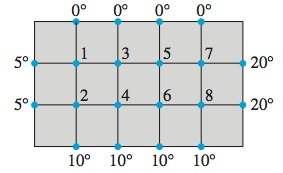
\includegraphics{https://raw.githubusercontent.com/zcczhang/Computational_Linear_Algebra/master/HW3/HWpic.jpeg}

An important concern in the study of heat transfer is to determine the
steady-state temperature distribution of a thin plate when the
temperature around the boundary is known. Assume the plate shown in the
figure above represents a cross section of a metal beam, with negligible
heat flow in the direction perpendicular to the plate. Let the variables
\(x_1, x_2, \ldots, x_8\) denote the temperatures at nodes 1 through 8
in the picture. In steady state, the temperature at a node is
approximately equal to the average of the four nearest nodes (to the
left, above, right, below).

\begin{enumerate}
\def\labelenumi{\alph{enumi})}
\item
  The solution to the approximate steady-state heat flow problem for
  this plate can be written as a system of linear equations \(Ax=b\),
  where \(x=[x_1, x_2, \ldots, x_8]\) is the vector of temperatures at
  nodes 1 through 8. Find the \(8 \times 8\) matrix \(A\) and the vector
  \(b\). Hint: \(A\) should be a banded matrix with many zeros in the
  top right and bottom left parts of \(A\).
\item
  Use your function from Exercise 1 (on the activity) to perform an LU
  factorization of \(A\). Do you notice anything special about the
  structures of \(L\) and \(U\)?
\item
  Once you have an LU factorization for a matrix \(A\), you need to do
  the two-step procedure to complete the back substitution to solve
  \(Ax=b\). Here is code for that:
\end{enumerate}

\begin{Shaded}
\begin{Highlighting}[]
\NormalTok{mySolve=}\ControlFlowTok{function}\NormalTok{(L,U,b,}\DataTypeTok{tol=}\FloatTok{1e-10}\NormalTok{)\{}

\NormalTok{  n=}\KeywordTok{nrow}\NormalTok{(L)}
  
  \CommentTok{# First solve Ly=b }
\NormalTok{  y =}\StringTok{ }\KeywordTok{rep}\NormalTok{(}\DecValTok{0}\NormalTok{,n)        }\CommentTok{# pre-allocate a vector y with 0s in it.}
  \ControlFlowTok{if}\NormalTok{(}\KeywordTok{abs}\NormalTok{(L[}\DecValTok{1}\NormalTok{,}\DecValTok{1}\NormalTok{])}\OperatorTok{<}\NormalTok{tol) }\KeywordTok{stop}\NormalTok{(}\StringTok{'There is a zero on the diagonal of L'}\NormalTok{)}
\NormalTok{  y[}\DecValTok{1}\NormalTok{] =}\StringTok{ }\NormalTok{b[}\DecValTok{1}\NormalTok{]}\OperatorTok{/}\NormalTok{L[}\DecValTok{1}\NormalTok{,}\DecValTok{1}\NormalTok{]  }\CommentTok{# Fill in the 1st value of y}
  \ControlFlowTok{for}\NormalTok{ (j }\ControlFlowTok{in} \DecValTok{2}\OperatorTok{:}\NormalTok{n ) \{}
    \ControlFlowTok{if}\NormalTok{(}\KeywordTok{abs}\NormalTok{(L[j,j])}\OperatorTok{<}\NormalTok{tol) }\KeywordTok{stop}\NormalTok{(}\StringTok{'There is a zero on the diagonal of L'}\NormalTok{)}
\NormalTok{    y[j] =}\StringTok{ }\NormalTok{(b[j] }\OperatorTok{-}\StringTok{ }\NormalTok{L[j,}\DecValTok{1}\OperatorTok{:}\NormalTok{(j}\DecValTok{-1}\NormalTok{)]}\OperatorTok\NormalTok{y[}\DecValTok{1}\OperatorTok{:}\NormalTok{(j}\DecValTok{-1}\NormalTok{)])}\OperatorTok{/}\NormalTok{L[j,j]}
\NormalTok{  \}}

  \CommentTok{# Then solve Ux=y }
\NormalTok{  x =}\StringTok{ }\KeywordTok{rep}\NormalTok{(}\DecValTok{0}\NormalTok{,n)        }\CommentTok{# pre-allocate a vector x with 0s in it.}
  \ControlFlowTok{if}\NormalTok{(}\KeywordTok{abs}\NormalTok{(U[n,n])}\OperatorTok{<}\NormalTok{tol) }\KeywordTok{stop}\NormalTok{(}\StringTok{'There is a zero on the diagonal of U'}\NormalTok{)}
\NormalTok{  x[n] =}\StringTok{ }\NormalTok{y[n]}\OperatorTok{/}\NormalTok{U[n,n]  }\CommentTok{# Fill in the nth value of x}
  \ControlFlowTok{for}\NormalTok{ (j }\ControlFlowTok{in}\NormalTok{ (n}\DecValTok{-1}\NormalTok{)}\OperatorTok{:}\DecValTok{1}\NormalTok{ ) \{}
    \ControlFlowTok{if}\NormalTok{(}\KeywordTok{abs}\NormalTok{(U[j,j])}\OperatorTok{<}\NormalTok{tol) }\KeywordTok{stop}\NormalTok{(}\StringTok{'There is a zero on the diagonal of U'}\NormalTok{)}
\NormalTok{    x[j] =}\StringTok{ }\NormalTok{(y[j] }\OperatorTok{-}\StringTok{ }\NormalTok{U[j,(j}\OperatorTok{+}\DecValTok{1}\NormalTok{)}\OperatorTok{:}\NormalTok{n]}\OperatorTok\NormalTok{x[(j}\OperatorTok{+}\DecValTok{1}\NormalTok{)}\OperatorTok{:}\NormalTok{n])}\OperatorTok{/}\NormalTok{U[j,j]}
\NormalTok{  \}}
  \KeywordTok{return}\NormalTok{(x)}
\NormalTok{\}}
\end{Highlighting}
\end{Shaded}

Make sure you understand what the code is doing, and then use it to find
the steady-state temperatures at nodes 1 through 8.

\begin{enumerate}
\def\labelenumi{\alph{enumi})}
\setcounter{enumi}{3}
\item
  The temperature on the right-hand side of the plate was measured
  incorrectly. It is actually 30 degrees. Find the new steady-state
  temperatures. Hint: you should not do another LU factorization!
\item
  Use the R function \texttt{solve(A)} to compute \(A^{-1}\). Note that
  \(A^{-1}\) is a \textbf{dense} matrix (without many zeros). When \(A\)
  is large, \(L\) and \(U\) can be stored in much less space than
  \(A^{-1}\). This fact is another reason for preferring the LU
  factorization of \(A\) to \(A^{-1}\) itself.
\end{enumerate}

\hypertarget{problem-3}{%
\subsubsection{Problem 3}\label{problem-3}}

\textbf{\emph{This problem is taken from the in-class portion of an old
midterm.}}

\textbf{You are trying to solve a linear system of four equations:}

\[\left[\begin{array}{ccc} && \\ & A &   \\ && \\ && \end{array}\right]
\left[\begin{array}{c}x_1 \\ x_2 \\ x_3 \\ x_4 \end{array}\right]=\left[\begin{array}{c}3 \\ -2 \\ 4 \\ 2.25 \end{array}\right]~,\]
\textbf{but unfortunately \(A\) is a black box and you cannot see the
contents. Oh my! Luckily, from the physics of the problem, you do have
three pieces of information about the system and the solution:}

\begin{itemize}
\item
  \(||x||_{\infty}=2\)
\item
  \textbf{The condition number of \(A\), using the \(\infty\)-norm, is
  32}
\item
  \textbf{\(\left[\begin{array}{ccc} && \\ & A & \\ && \\ && \end{array}\right] \left[\begin{array}{r}2.0750 \\ 0.1625 \\ 0.4500 \\ -0.1875 \end{array}\right]=\left[\begin{array}{c}3 \\ -2 \\ 4 \\ 2.1875 \end{array}\right]\)}
\end{itemize}

\textbf{Is this information enough to determine the solution \(x\) to
\(Ax=b\)? If yes, find \(x\). If no, say as much as you can about
\(x\).}

\emph{solution}

\begin{quote}
\[
Cond(A)=||A||_{\infty}||A^{-1}||_{\infty}=32=\max\frac{\text { relative forward error }}{\text { relative backward error }}=\max\frac{\frac{\left\|x-x_{a}\right\|_{\infty}}{\|x\|_{\infty}}}{\frac{\left\|A x_{a}-b\right\|_{\infty}}{\|b\|_{\infty}}}=\max\frac{\frac{\left\|x-x_{a}\right\|_{\infty}}{2}}{\frac{|2.25-2.1875|}{4}}
\]
\end{quote}

\begin{Shaded}
\begin{Highlighting}[]
\DecValTok{32}\OperatorTok{*}\NormalTok{(}\FloatTok{2.25-2.1875}\NormalTok{)}\OperatorTok{/}\DecValTok{2}
\end{Highlighting}
\end{Shaded}

\begin{verbatim}
## [1] 1
\end{verbatim}

\begin{quote}
\[
\therefore ||x-x_{a}||_{\infty} \leq 1\\
\because ||x||_{\infty} = 2 = \max\{|\bar{x}|\} \text{ and } x_{a}=\left[\begin{array}{c}2.0750 \\ 0.1625 \\ 0.4500 \\ -0.1875 \end{array}\right]\\
\therefore |x_{i}-x_{ai}|\leq 1 \; i=1,2,3,4 \\
\therefore |x_{1}|=2\\
\text{and:  } 
\begin{aligned}-0.8375 & \leq x_{2} \leq 1.1625 \\-0.55 & \leq x_{3} \leq 1.45 \\-1.1875 & \leq x_{4} \leq 0.8125 \end{aligned}
\]
\end{quote}

\begin{quote}
I believe this is what we can find for \(x\)
\end{quote}

\hypertarget{problem-4}{%
\subsubsection{Problem 4}\label{problem-4}}

A real \(n \times n\) matrix \(Q\) is \emph{orthonormal} if

\[ Q^{\top}Q=QQ^T=I;~i.e., Q^{-1}=Q^T.\]

Note: sometimes you will see these matrices just called \emph{orthogonal
matrices}. The analagous matrices that contain complex entries
(\(Q^*Q=QQ^*=I\), where the \(~^*\) is a conjugate transpose) are called
\emph{unitary}.

Show that \(||Q||_2=||Q^{-1}||_2=1\), and therefore the 2-norm condition
number of any orthonormal matrix \(Q\) is
\(\kappa_2(Q)=||Q||_2 ||Q^{-1}||_2=1\).

\hypertarget{problem-5}{%
\subsubsection{Problem 5}\label{problem-5}}

This problem has 3 parts.

\begin{enumerate}
\def\labelenumi{(\alph{enumi})}
\tightlist
\item
  Modify my \texttt{UnitCircleMap} function, which shows the image of
  the unit ball under a linear mapping \(A\) and computes the matrix
  norm of \(A\). We want to let the user choose the norm to be 1, 2, or
  \(\infty\) (``I''). The code is below, and there are a few places
  where you need to insert a few lines.
\end{enumerate}

\begin{Shaded}
\begin{Highlighting}[]
\NormalTok{UnitCircleMap =}\StringTok{ }\ControlFlowTok{function}\NormalTok{(A,}\DataTypeTok{p=}\DecValTok{2}\NormalTok{) \{}
  
  \ControlFlowTok{if}\NormalTok{ (p}\OperatorTok{==}\DecValTok{2}\NormalTok{) \{}
\NormalTok{    t =}\StringTok{ }\KeywordTok{seq}\NormalTok{(}\DecValTok{0}\NormalTok{,}\DecValTok{2}\OperatorTok{*}\NormalTok{pi,}\DataTypeTok{len=}\DecValTok{1000}\NormalTok{)}
\NormalTok{    x =}\StringTok{ }\KeywordTok{cos}\NormalTok{(t)}
\NormalTok{    y =}\StringTok{ }\KeywordTok{sin}\NormalTok{(t)}
\NormalTok{    nn=}\KeywordTok{norm}\NormalTok{(A,}\DataTypeTok{type=}\StringTok{"2"}\NormalTok{)}
\NormalTok{    ni=}\KeywordTok{as.character}\NormalTok{(p)}
\NormalTok{  \}}
  \ControlFlowTok{else} \ControlFlowTok{if}\NormalTok{ (p}\OperatorTok{==}\DecValTok{1}\NormalTok{)\{}
    \CommentTok{# Insert some code here to create points along the unit 1-norm circle}
\NormalTok{    x=}\KeywordTok{c}\NormalTok{(}\KeywordTok{seq}\NormalTok{(}\DecValTok{1}\NormalTok{,}\DecValTok{0}\NormalTok{,}\DataTypeTok{len=}\DecValTok{500}\NormalTok{),}\KeywordTok{seq}\NormalTok{(}\DecValTok{0}\NormalTok{,}\OperatorTok{-}\DecValTok{1}\NormalTok{,}\DataTypeTok{len=}\DecValTok{500}\NormalTok{),}\KeywordTok{seq}\NormalTok{(}\OperatorTok{-}\DecValTok{1}\NormalTok{,}\DecValTok{0}\NormalTok{,}\DataTypeTok{len=}\DecValTok{500}\NormalTok{),}\KeywordTok{seq}\NormalTok{(}\DecValTok{0}\NormalTok{,}\DecValTok{1}\NormalTok{,}\DataTypeTok{len=}\DecValTok{500}\NormalTok{))}
\NormalTok{    y=}\KeywordTok{c}\NormalTok{(}\KeywordTok{seq}\NormalTok{(}\DecValTok{0}\NormalTok{,}\DecValTok{1}\NormalTok{,}\DataTypeTok{len=}\DecValTok{500}\NormalTok{),}\KeywordTok{seq}\NormalTok{(}\DecValTok{1}\NormalTok{,}\DecValTok{0}\NormalTok{,}\DataTypeTok{len=}\DecValTok{500}\NormalTok{),}\KeywordTok{seq}\NormalTok{(}\DecValTok{0}\NormalTok{,}\OperatorTok{-}\DecValTok{1}\NormalTok{,}\DataTypeTok{len=}\DecValTok{500}\NormalTok{),}\KeywordTok{seq}\NormalTok{(}\OperatorTok{-}\DecValTok{1}\NormalTok{,}\DecValTok{0}\NormalTok{,}\DataTypeTok{len=}\DecValTok{500}\NormalTok{))}
\NormalTok{    nn=}\KeywordTok{norm}\NormalTok{(A,}\DataTypeTok{type=}\StringTok{"1"}\NormalTok{)}
\NormalTok{    ni=}\KeywordTok{as.character}\NormalTok{(p)}
\NormalTok{  \}}
  \ControlFlowTok{else} \ControlFlowTok{if}\NormalTok{ (p}\OperatorTok{==}\StringTok{"I"}\NormalTok{)\{}
    \CommentTok{# Insert some code here to create points along the unit infinity-norm circle}
\NormalTok{    x=}\KeywordTok{c}\NormalTok{(}\KeywordTok{rep}\NormalTok{(}\DecValTok{1}\NormalTok{,}\DecValTok{500}\NormalTok{),}\KeywordTok{seq}\NormalTok{(}\DecValTok{1}\NormalTok{,}\OperatorTok{-}\DecValTok{1}\NormalTok{,}\DataTypeTok{len=}\DecValTok{500}\NormalTok{),}\KeywordTok{rep}\NormalTok{(}\OperatorTok{-}\DecValTok{1}\NormalTok{,}\DecValTok{500}\NormalTok{),}\KeywordTok{seq}\NormalTok{(}\OperatorTok{-}\DecValTok{1}\NormalTok{,}\DecValTok{1}\NormalTok{,}\DataTypeTok{len=}\DecValTok{500}\NormalTok{))}
\NormalTok{    y=}\KeywordTok{c}\NormalTok{(}\KeywordTok{seq}\NormalTok{(}\OperatorTok{-}\DecValTok{1}\NormalTok{,}\DecValTok{1}\NormalTok{,}\DataTypeTok{len=}\DecValTok{500}\NormalTok{),}\KeywordTok{rep}\NormalTok{(}\DecValTok{1}\NormalTok{,}\DecValTok{500}\NormalTok{),}\KeywordTok{seq}\NormalTok{(}\DecValTok{1}\NormalTok{,}\OperatorTok{-}\DecValTok{1}\NormalTok{,}\DataTypeTok{len=}\DecValTok{500}\NormalTok{),}\KeywordTok{rep}\NormalTok{(}\OperatorTok{-}\DecValTok{1}\NormalTok{,}\DecValTok{500}\NormalTok{))}
\NormalTok{    nn=}\KeywordTok{norm}\NormalTok{(A,}\DataTypeTok{type=}\StringTok{"I"}\NormalTok{)}
\NormalTok{    ni=}\StringTok{"Inf"}
\NormalTok{  \}}
  
\NormalTok{  pts =}\StringTok{ }\NormalTok{A }\OperatorTok\StringTok{ }\KeywordTok{t}\NormalTok{(}\KeywordTok{cbind}\NormalTok{(x,y))}
  
\NormalTok{  newx =}\StringTok{ }\NormalTok{pts[}\DecValTok{1}\NormalTok{,]}
\NormalTok{  newy =}\StringTok{ }\NormalTok{pts[}\DecValTok{2}\NormalTok{,]}
  
\NormalTok{  M =}\StringTok{ }\KeywordTok{max}\NormalTok{(}\KeywordTok{c}\NormalTok{(newx,newy,}\FloatTok{1.5}\NormalTok{))}
\NormalTok{  m =}\StringTok{ }\KeywordTok{min}\NormalTok{(}\KeywordTok{c}\NormalTok{(newx,newy,}\OperatorTok{-}\FloatTok{1.5}\NormalTok{))}
  
  \KeywordTok{plot}\NormalTok{(x,y,}\DataTypeTok{type=}\StringTok{'l'}\NormalTok{,}\DataTypeTok{col=}\StringTok{'black'}\NormalTok{,}\DataTypeTok{xlim=}\KeywordTok{c}\NormalTok{(m,M),}\DataTypeTok{ylim=}\KeywordTok{c}\NormalTok{(m,M),}\DataTypeTok{xlab=}\StringTok{"x1"}\NormalTok{,}\DataTypeTok{ylab=}\StringTok{"x2"}\NormalTok{)}
  \KeywordTok{lines}\NormalTok{(newx,newy,}\DataTypeTok{col=}\StringTok{'red'}\NormalTok{)}
  
\NormalTok{  normSize=}\KeywordTok{sprintf}\NormalTok{(}\StringTok{"||A||_%s = %1.2f"}\NormalTok{,ni,nn)}
  \KeywordTok{text}\NormalTok{(}\OperatorTok{-}\NormalTok{.}\DecValTok{7}\OperatorTok{*}\NormalTok{M,.}\DecValTok{9}\OperatorTok{*}\NormalTok{M,normSize)}
\NormalTok{\}}
\end{Highlighting}
\end{Shaded}

Here is an example of how the function should be called, and the output
it should display. In this case,
\(A=\begin{bmatrix}1 & 2 \\ 0 & 2\end{bmatrix}\). Once you've filled in
the missing lines of the function, you can also test your code on this
\(A\) with the 1 norm and \(\infty\)-norm.

\begin{Shaded}
\begin{Highlighting}[]
\NormalTok{A=}\KeywordTok{cbind}\NormalTok{(}\KeywordTok{c}\NormalTok{(}\DecValTok{1}\NormalTok{,}\DecValTok{0}\NormalTok{),}\KeywordTok{c}\NormalTok{(}\DecValTok{2}\NormalTok{,}\DecValTok{2}\NormalTok{))}
\KeywordTok{UnitCircleMap}\NormalTok{(A,}\DataTypeTok{p=}\DecValTok{2}\NormalTok{)}
\end{Highlighting}
\end{Shaded}

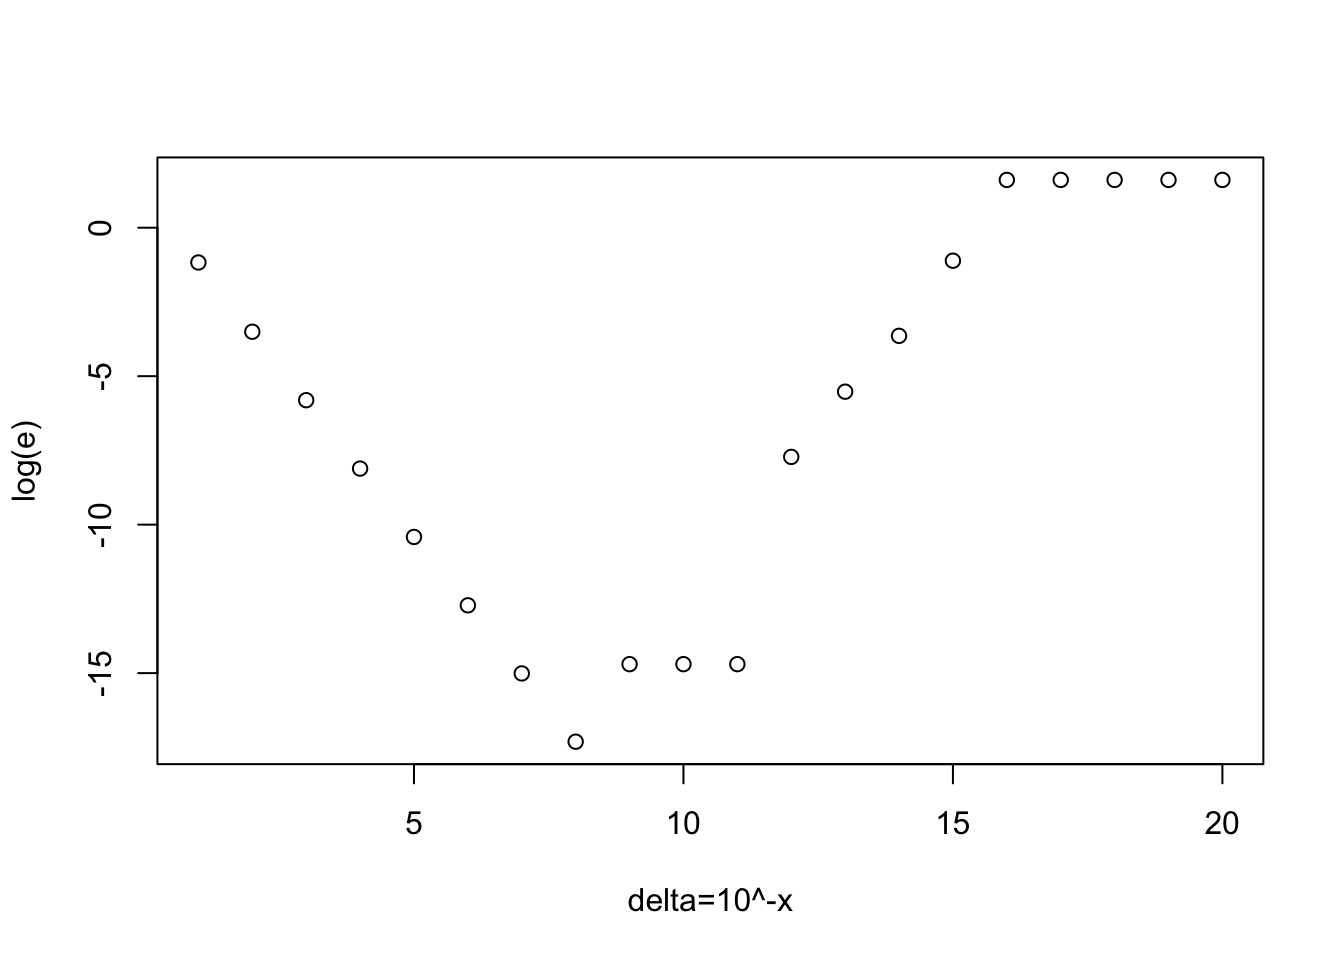
\includegraphics{365_HW3_files/figure-latex/unnamed-chunk-6-1.pdf}

\begin{Shaded}
\begin{Highlighting}[]
\NormalTok{A=}\KeywordTok{cbind}\NormalTok{(}\KeywordTok{c}\NormalTok{(}\DecValTok{1}\NormalTok{,}\DecValTok{0}\NormalTok{),}\KeywordTok{c}\NormalTok{(}\DecValTok{2}\NormalTok{,}\DecValTok{2}\NormalTok{))}
\KeywordTok{UnitCircleMap}\NormalTok{(A,}\DataTypeTok{p=}\DecValTok{1}\NormalTok{)}
\end{Highlighting}
\end{Shaded}

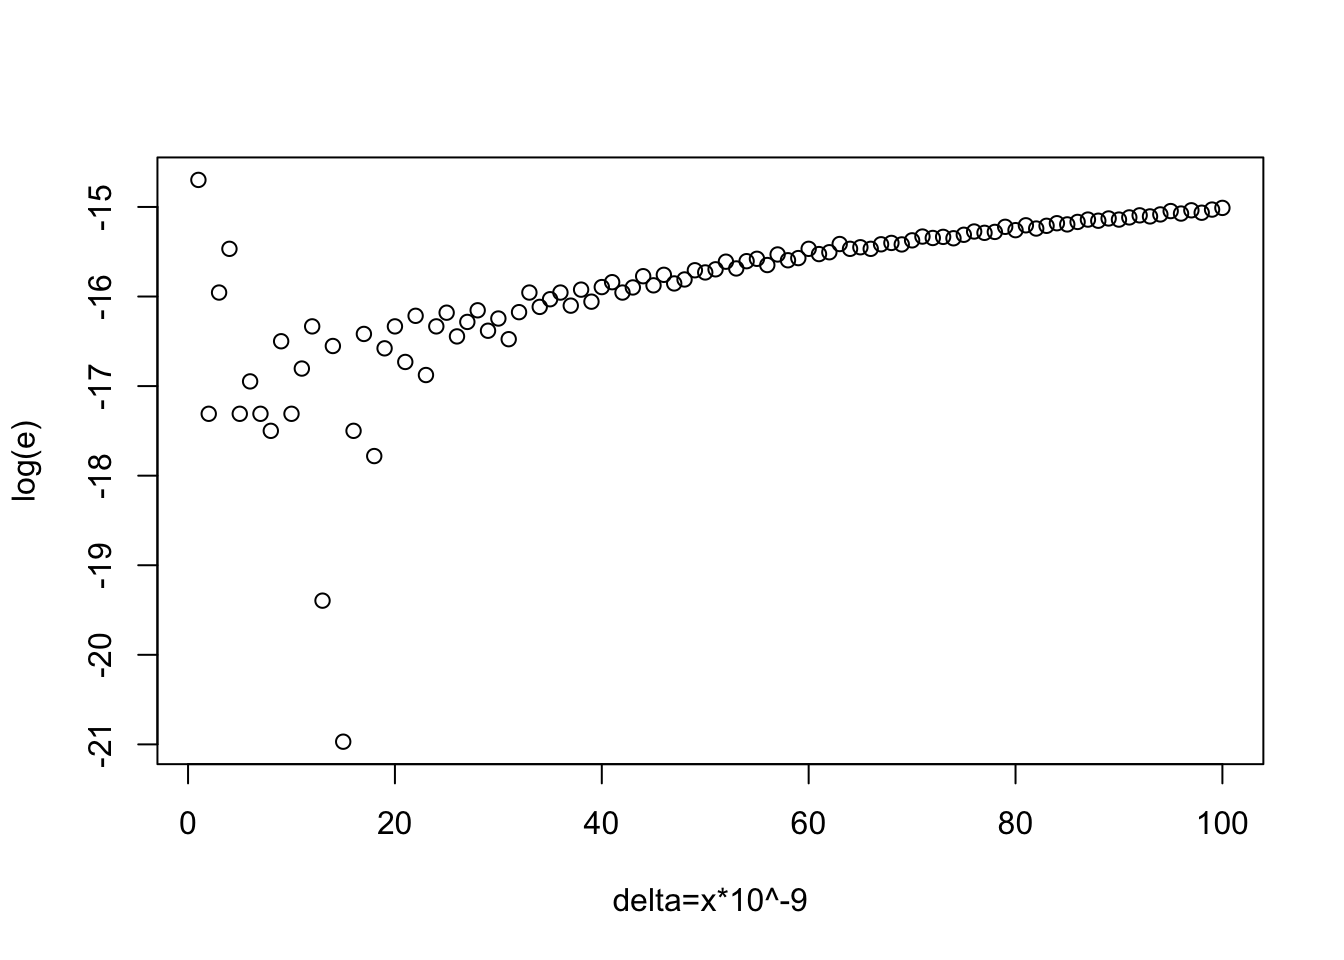
\includegraphics{365_HW3_files/figure-latex/unnamed-chunk-6-2.pdf}

\begin{Shaded}
\begin{Highlighting}[]
\NormalTok{A=}\KeywordTok{cbind}\NormalTok{(}\KeywordTok{c}\NormalTok{(}\DecValTok{1}\NormalTok{,}\DecValTok{0}\NormalTok{),}\KeywordTok{c}\NormalTok{(}\DecValTok{2}\NormalTok{,}\DecValTok{2}\NormalTok{))}
\KeywordTok{UnitCircleMap}\NormalTok{(A,}\DataTypeTok{p=}\StringTok{'I'}\NormalTok{)}
\end{Highlighting}
\end{Shaded}

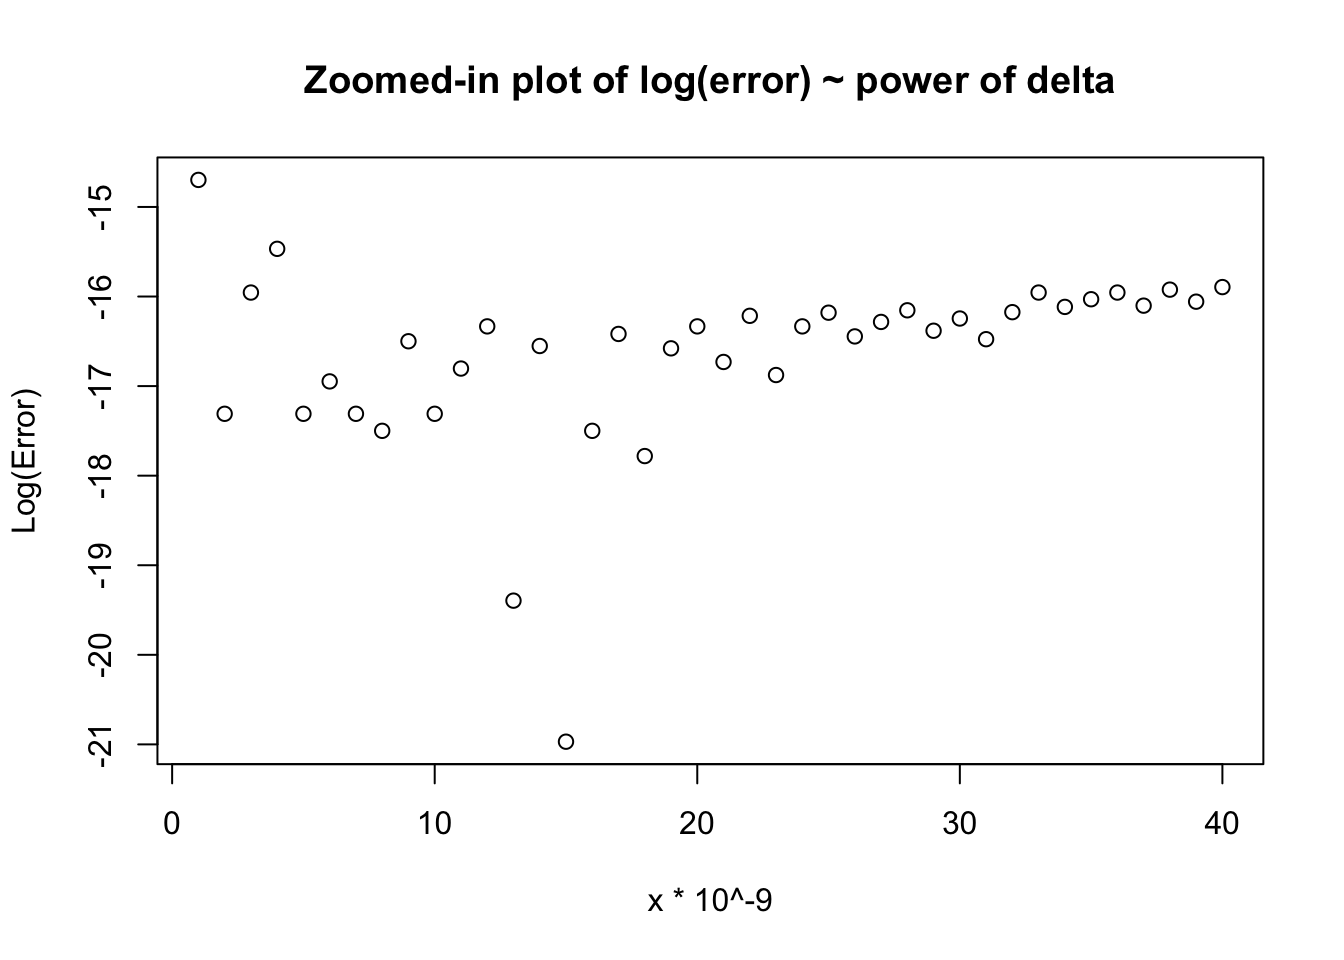
\includegraphics{365_HW3_files/figure-latex/unnamed-chunk-6-3.pdf}

\begin{enumerate}
\def\labelenumi{(\alph{enumi})}
\setcounter{enumi}{1}
\tightlist
\item
  Compute the condition number of the matrix \(A\) above using
  \texttt{Cond} (using the \(p=1,2, \infty\)-norms). Visually explain
  why the condition number for each \(p\) is the value you found.
\end{enumerate}

\begin{Shaded}
\begin{Highlighting}[]
\NormalTok{Cond =}\StringTok{ }\ControlFlowTok{function}\NormalTok{(A,}\DataTypeTok{p=}\DecValTok{2}\NormalTok{) \{}
  \ControlFlowTok{if}\NormalTok{ (p }\OperatorTok{==}\StringTok{ }\DecValTok{2}\NormalTok{) \{  }\CommentTok{# by default use the }
\NormalTok{    s =}\StringTok{ }\KeywordTok{svd}\NormalTok{(A)}\OperatorTok{$}\NormalTok{d}
\NormalTok{    s =}\StringTok{ }\NormalTok{s[s}\OperatorTok{>}\DecValTok{0}\NormalTok{]}
    \KeywordTok{return}\NormalTok{(}\KeywordTok{max}\NormalTok{(s)}\OperatorTok{/}\KeywordTok{min}\NormalTok{(s))}
\NormalTok{  \}}
  \ControlFlowTok{if}\NormalTok{ (p }\OperatorTok{==}\StringTok{ }\DecValTok{1}\NormalTok{) \{  }\CommentTok{# use the 1 norm}
\NormalTok{    Ainv =}\StringTok{ }\KeywordTok{solve}\NormalTok{(A)}
    \KeywordTok{return}\NormalTok{(}\KeywordTok{max}\NormalTok{(}\KeywordTok{colSums}\NormalTok{(}\KeywordTok{abs}\NormalTok{(A)))}\OperatorTok{*}\KeywordTok{max}\NormalTok{(}\KeywordTok{colSums}\NormalTok{(}\KeywordTok{abs}\NormalTok{(Ainv))))}
\NormalTok{  \}}
  \ControlFlowTok{if}\NormalTok{ (p }\OperatorTok{==}\StringTok{ 'I'}\NormalTok{) \{   }\CommentTok{# use the infinity norm}
\NormalTok{    Ainv =}\StringTok{ }\KeywordTok{solve}\NormalTok{(A)}
    \KeywordTok{return}\NormalTok{(}\KeywordTok{max}\NormalTok{(}\KeywordTok{rowSums}\NormalTok{(}\KeywordTok{abs}\NormalTok{(A)))}\OperatorTok{*}\KeywordTok{max}\NormalTok{(}\KeywordTok{rowSums}\NormalTok{(}\KeywordTok{abs}\NormalTok{(Ainv))))}
\NormalTok{  \}}
\NormalTok{\}}
\end{Highlighting}
\end{Shaded}

\begin{Shaded}
\begin{Highlighting}[]
\NormalTok{A=}\KeywordTok{cbind}\NormalTok{(}\KeywordTok{c}\NormalTok{(}\DecValTok{1}\NormalTok{,}\DecValTok{0}\NormalTok{),}\KeywordTok{c}\NormalTok{(}\DecValTok{2}\NormalTok{,}\DecValTok{2}\NormalTok{))}
\KeywordTok{Cond}\NormalTok{(A,}\DecValTok{1}\NormalTok{)}
\end{Highlighting}
\end{Shaded}

\begin{verbatim}
## [1] 6
\end{verbatim}

\begin{Shaded}
\begin{Highlighting}[]
\KeywordTok{Cond}\NormalTok{(A,}\DecValTok{2}\NormalTok{)}
\end{Highlighting}
\end{Shaded}

\begin{verbatim}
## [1] 4.265564
\end{verbatim}

\begin{Shaded}
\begin{Highlighting}[]
\KeywordTok{Cond}\NormalTok{(A,}\StringTok{"I"}\NormalTok{)}
\end{Highlighting}
\end{Shaded}

\begin{verbatim}
## [1] 6
\end{verbatim}

\begin{enumerate}
\def\labelenumi{(\alph{enumi})}
\setcounter{enumi}{2}
\tightlist
\item
  Use your code to determine whether
  \(||Q||_1=||Q||_{\infty}=||Q||_2=1\) for all orthonormal matrices
  \(Q\).
\end{enumerate}

\textbf{Hint}: Try
\(Q=\begin{pmatrix} \frac{1}{\sqrt{2}} & \frac{-1}{\sqrt{2}} \\ \frac{1}{\sqrt{2}} & \frac{1}{\sqrt{2}} \end{pmatrix}\),
which is a rotation matrix that rotates vectors counter-clockwise by
\(\frac{\pi}{4}\).

\begin{Shaded}
\begin{Highlighting}[]
\NormalTok{A=}\KeywordTok{cbind}\NormalTok{(}\KeywordTok{c}\NormalTok{(}\DecValTok{1}\OperatorTok{/}\KeywordTok{sqrt}\NormalTok{(}\DecValTok{2}\NormalTok{),}\DecValTok{1}\OperatorTok{/}\KeywordTok{sqrt}\NormalTok{(}\DecValTok{2}\NormalTok{)),}\KeywordTok{c}\NormalTok{(}\OperatorTok{-}\DecValTok{1}\OperatorTok{/}\KeywordTok{sqrt}\NormalTok{(}\DecValTok{2}\NormalTok{),}\DecValTok{1}\OperatorTok{/}\KeywordTok{sqrt}\NormalTok{(}\DecValTok{2}\NormalTok{)))}
\KeywordTok{UnitCircleMap}\NormalTok{(A,}\DataTypeTok{p=}\DecValTok{1}\NormalTok{)}
\end{Highlighting}
\end{Shaded}

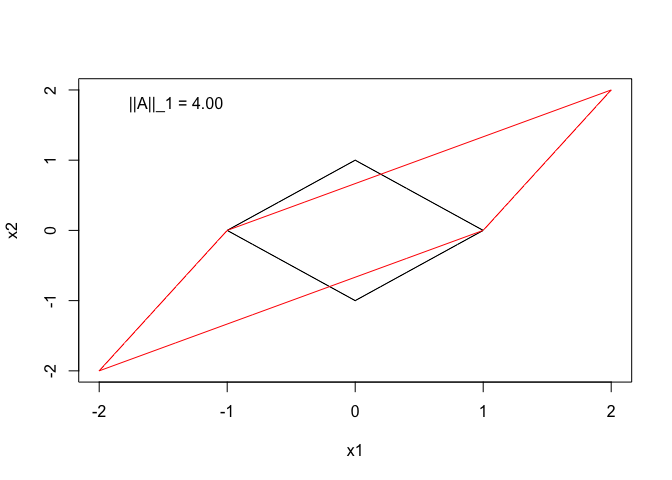
\includegraphics{365_HW3_files/figure-latex/unnamed-chunk-9-1.pdf}

\begin{Shaded}
\begin{Highlighting}[]
\KeywordTok{UnitCircleMap}\NormalTok{(A,}\DataTypeTok{p=}\DecValTok{2}\NormalTok{)}
\end{Highlighting}
\end{Shaded}

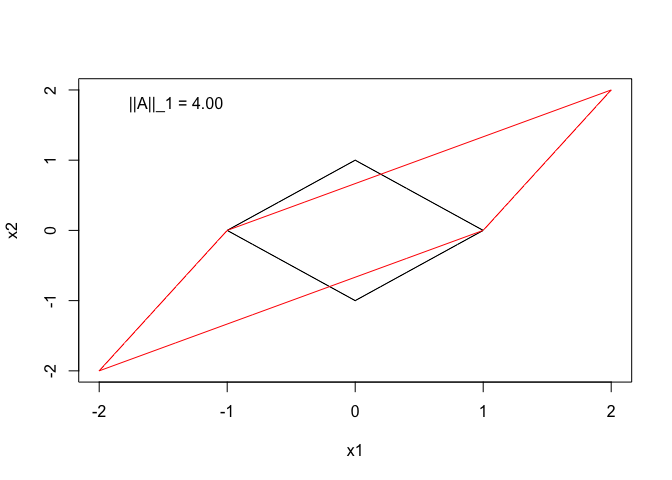
\includegraphics{365_HW3_files/figure-latex/unnamed-chunk-9-2.pdf}

\begin{Shaded}
\begin{Highlighting}[]
\KeywordTok{UnitCircleMap}\NormalTok{(A,}\DataTypeTok{p=}\StringTok{"I"}\NormalTok{)}
\end{Highlighting}
\end{Shaded}

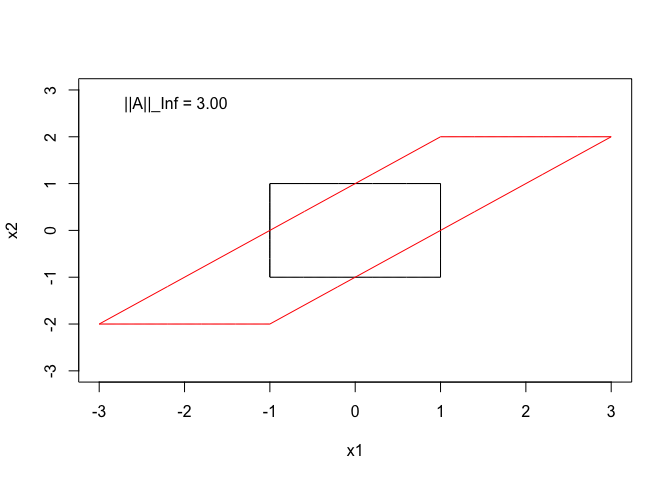
\includegraphics{365_HW3_files/figure-latex/unnamed-chunk-9-3.pdf}

\begin{quote}
Therefore, they are not necessarily equal to 1.
\end{quote}

\hypertarget{problem-6}{%
\subsubsection{Problem 6}\label{problem-6}}

This was Question 5 on the Activity on norms.

Prove that
\[ ||A||_{\infty}=\max_{1 \leq i \leq n}\left\{ \sum_{j=1}^n |A_{ij}| \right\}=\text{maximum absolute row sum}.\]

\BeginKnitrBlock{proof}

\iffalse{} {Proof. } \fi{}\[
\because ||x||_{\infty} = \max_{1 \leq i\leq n}\{|\bar{x_i}|\}\\
\therefore ||A||_{\infty}=\max_{||x||_{\infty}=1}\{||Ax||_{\infty}\}=\max_{||x||_{\infty}=1}\max_{1 \leq i \leq n}\{\sum^{n}_{j=1}|A_{ij}x_{j}|\}=\max_{1 \leq i \leq n}\max_{||x||_{\infty}=1}\{\sum^{n}_{j=1}|A_{ij}x_{j}|\} \\= 
\max_{1 \leq i \leq n}\left\{ \sum_{j=1}^n |A_{ij}| \right\}=\text{maximum absolute row sum}.
\]

\EndKnitrBlock{proof}

\hypertarget{problem-7}{%
\subsubsection{Problem 7}\label{problem-7}}

Solve the following system by finding the \(PA=LU\) factorization and
then carrying out the two-step back substitution (all by hand, that is,
not using any R functions. Of course, you can type your solution, and
check your work in R, though.):

\[ Ax=\begin{pmatrix}-1 & 0 & 1 \\
3 & 1 & 1 \\
2 & 0 & 1 
\end{pmatrix} \begin{pmatrix} x_1 \\ x_2\\ x_3\end{pmatrix}=\begin{pmatrix} 2 \\ 5 \\ 5 \end{pmatrix}=b. \]

\BeginKnitrBlock{solution}

\iffalse{} {Solution. } \fi{}\[
U = A = \begin{pmatrix}-1 & 0 & 1 \\
3 & 1 & 1 \\
2 & 0 & 1 
\end{pmatrix}\text{, } P = I =\left(\begin{array}{ccc}{1} & {0} & {0} \\ {0} & {1} & {0} \\ {0} & {0} & {1}\end{array}\right) \\
\text{exchange the first two rows: }U  = \begin{pmatrix}3 & 1 & 1 \\-1 & 0 & 1 \\
2 & 0 & 1 
\end{pmatrix} \text{, } P  =\left(\begin{array}{ccc}{0} & {1} & {0} \\ {1} & {0} & {0} \\ {0} & {0} & {1}\end{array}\right)\\
\] \[
U = \left(\begin{array}{ccc}{3} & {1} & {1} \\ {-1} & {0} & {1} \\ {2} & {0} & {1}\end{array}\right) \frac{row2=\frac{1}{3} row1+row2}{row3=row3-\frac{2}{3} row1}\left(\begin{array}{rrr}{3} & {1} & {1} \\ {0} & {\frac{1}{3}} & {\frac{4}{3}} \\ {0} & {-\frac{2}{3}} & {\frac{1}{3}}\end{array}\right)
\] \[
L=\left(\begin{array}{ccc}{1} & {0} & {0} \\ {-\frac{1}{3}} & {1} & {0} \\ {\frac{2}{3}} & {0} & {1}\end{array}\right) \quad P=\left(\begin{array}{ccc}{0} & {1} & {0} \\ {1} & {0} & {0} \\ {0} & {0} & {1}\end{array}\right)
\] \[
s
\]

\EndKnitrBlock{solution}

\begin{Shaded}
\begin{Highlighting}[]
\NormalTok{P =}\StringTok{ }\KeywordTok{cbind}\NormalTok{(}\KeywordTok{c}\NormalTok{(}\DecValTok{0}\NormalTok{,}\DecValTok{1}\NormalTok{,}\DecValTok{0}\NormalTok{),}\KeywordTok{c}\NormalTok{(}\DecValTok{1}\NormalTok{,}\DecValTok{0}\NormalTok{,}\DecValTok{0}\NormalTok{),}\KeywordTok{c}\NormalTok{(}\DecValTok{0}\NormalTok{,}\DecValTok{0}\NormalTok{,}\DecValTok{1}\NormalTok{))}
\NormalTok{A =}\StringTok{ }\KeywordTok{rbind}\NormalTok{(}\KeywordTok{c}\NormalTok{(}\OperatorTok{-}\DecValTok{1}\NormalTok{,}\DecValTok{0}\NormalTok{,}\DecValTok{1}\NormalTok{),}\KeywordTok{c}\NormalTok{(}\DecValTok{3}\NormalTok{,}\DecValTok{1}\NormalTok{,}\DecValTok{1}\NormalTok{),}\KeywordTok{c}\NormalTok{(}\DecValTok{2}\NormalTok{,}\DecValTok{0}\NormalTok{,}\DecValTok{1}\NormalTok{))}
\NormalTok{L =}\StringTok{ }\KeywordTok{cbind}\NormalTok{(}\KeywordTok{c}\NormalTok{(}\DecValTok{1}\NormalTok{,}\OperatorTok{-}\DecValTok{1}\OperatorTok{/}\DecValTok{3}\NormalTok{,}\DecValTok{0}\NormalTok{),}\KeywordTok{c}\NormalTok{(}\DecValTok{0}\NormalTok{,}\DecValTok{1}\NormalTok{,}\DecValTok{2}\NormalTok{),}\KeywordTok{c}\NormalTok{(}\DecValTok{0}\NormalTok{,}\DecValTok{0}\NormalTok{,}\DecValTok{1}\NormalTok{))}
\NormalTok{U =}\StringTok{ }\KeywordTok{cbind}\NormalTok{(}\KeywordTok{c}\NormalTok{(}\DecValTok{3}\NormalTok{,}\DecValTok{0}\NormalTok{,}\DecValTok{0}\NormalTok{),}\KeywordTok{c}\NormalTok{(}\DecValTok{1}\NormalTok{,}\DecValTok{1}\OperatorTok{/}\DecValTok{3}\NormalTok{,}\DecValTok{0}\NormalTok{),}\KeywordTok{c}\NormalTok{(}\DecValTok{1}\NormalTok{,}\DecValTok{4}\OperatorTok{/}\DecValTok{3}\NormalTok{,}\DecValTok{3}\NormalTok{))}
\NormalTok{P }\OperatorTok\StringTok{ }\NormalTok{A}
\end{Highlighting}
\end{Shaded}

\begin{verbatim}
##      [,1] [,2] [,3]
## [1,]    3    1    1
## [2,]   -1    0    1
## [3,]    2    0    1
\end{verbatim}

\begin{Shaded}
\begin{Highlighting}[]
\NormalTok{L }\OperatorTok\StringTok{ }\NormalTok{U}
\end{Highlighting}
\end{Shaded}

\begin{verbatim}
##      [,1]      [,2]     [,3]
## [1,]    3 1.0000000 1.000000
## [2,]   -1 0.0000000 1.000000
## [3,]    0 0.6666667 5.666667
\end{verbatim}

\[
\begin{array}{l}{\left(\begin{array}{ccc}{1} & {0} & {0} \\ {\frac{2}{3}} & {1} & {0} \\ {-\frac{1}{3}} & {-\frac{1}{2}} & {1}\end{array}\right)(y)=\left(\begin{array}{l}{5} \\ {5} \\ {2}\end{array}\right) \Rightarrow y=\left(\begin{array}{c}{5} \\ {\frac{5}{3}} \\ {\frac{9}{2}}\end{array}\right)} \\ {\left(\begin{array}{ccc}{3} & {1} & {1} \\ {0} & {-\frac{2}{3}} & {\frac{1}{3}} \\ {0} & {0} & {1.5}\end{array}\right)(x)=\left(\begin{array}{c}{5} \\ {\frac{5}{3}} \\ {\frac{9}{2}}\end{array}\right) \Rightarrow x=\left(\begin{array}{c}{1} \\ {-1} \\ {3}\end{array}\right)}\end{array}
\]

\end{document}
